% !TeX spellcheck = en-GB
\section{Results}
The five fold cross validation of the proposed algorithm yields a mean DICE of $0.91$ with a standard deviation of $0.03$. This can be graphically seen in \autoref{fig:dicecrossvalid}. The range lies between $0.85$ and $0.96$ and has a median of $0.9$. The average computation time for the whole algorithm is $2.5$ minutes. Additionally one can see, that the post processing increases the results by $0.05$ on average.
\begin{figure}[h]
\centering
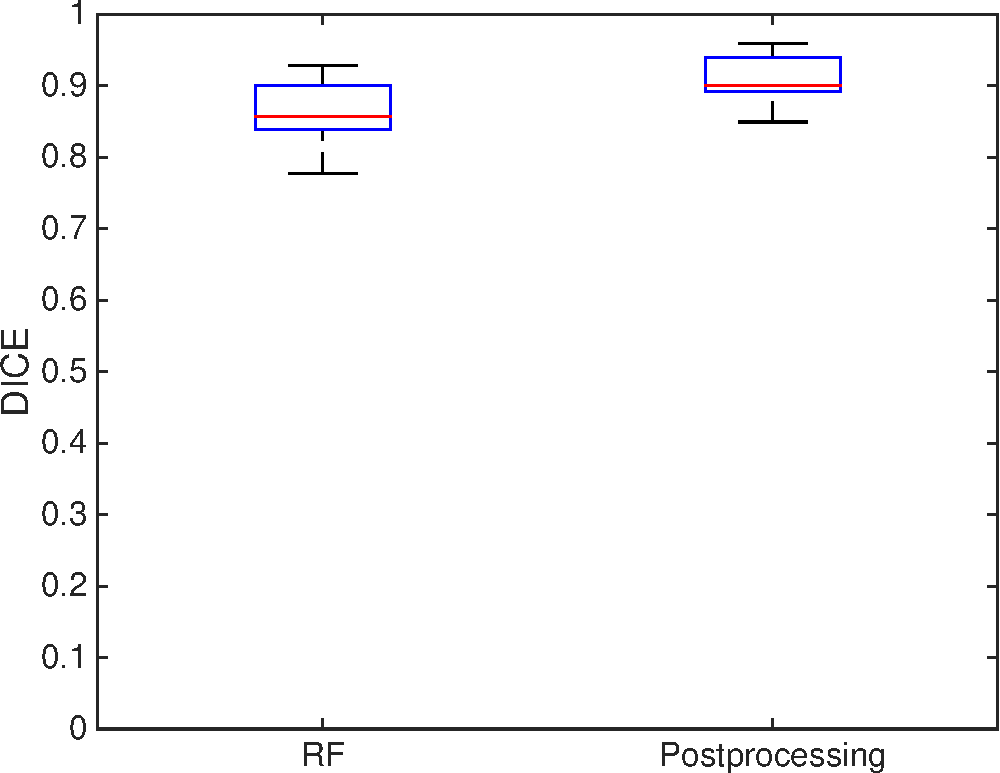
\includegraphics[width=0.9\linewidth]{dicecrossvalid.pdf}
\caption{DICE}
\label{fig:dicecrossvalid}
\end{figure}

In \autoref{fig:bestcase} and \autoref{fig:worstcase} the optically best and worst result out of the second data set are shown. These are based on objective observations and not on quantitative measures, as we do not have the ground truth to this data.
\begin{figure*}[!t]
	\centering
	\subfloat[Bestcase result of the test data (Image 29)]{
		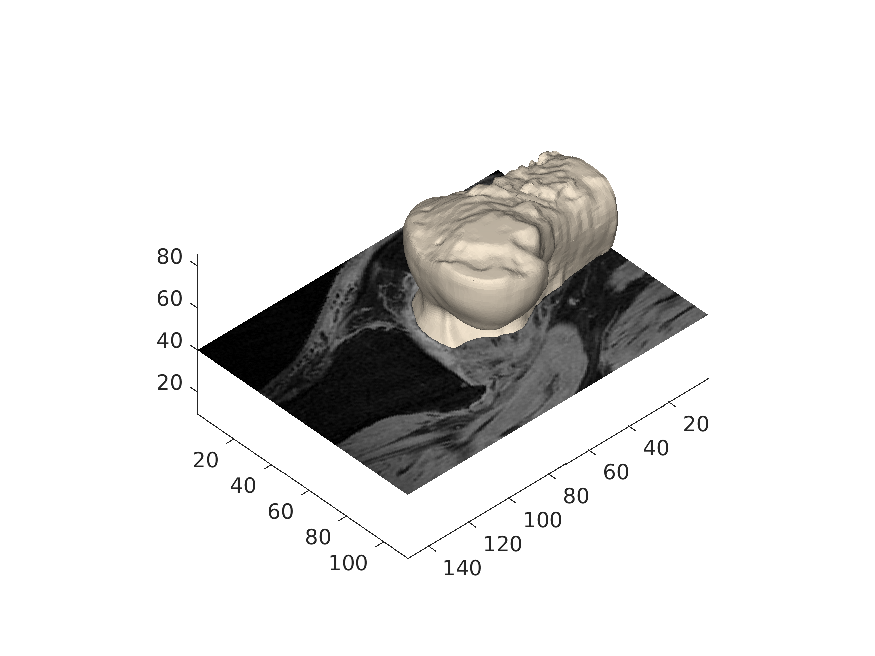
\includegraphics[width=0.48\textwidth]{vr029}
		\label{fig:bestcase}}
	\hfil
	\subfloat[Worstcase result of the test data (Image 21)]{
		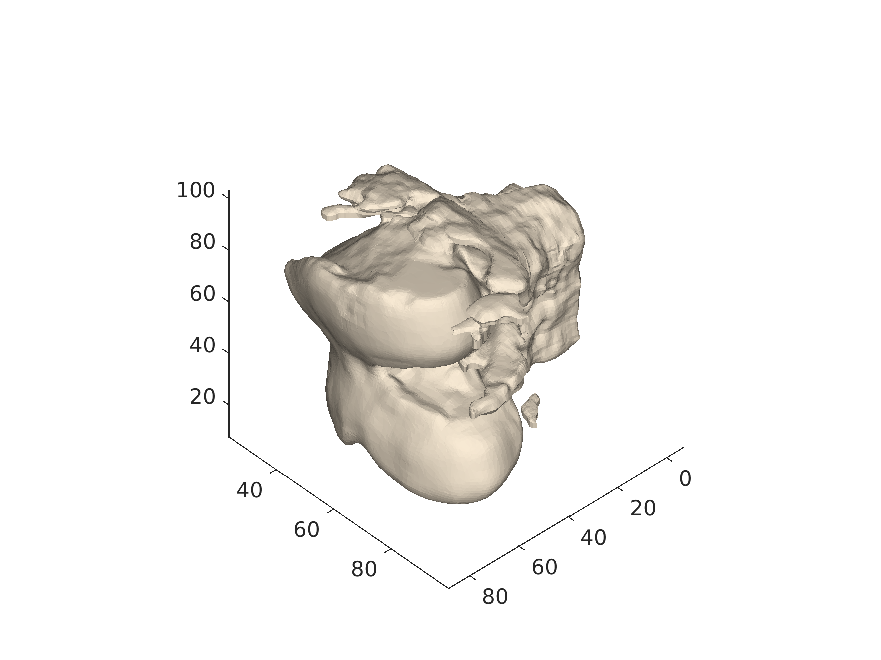
\includegraphics[width=0.48\textwidth]{vr021}
		\label{fig:worstcase}}
\end{figure*}